\documentclass{standalone}
\usepackage{pgfplots}
\pgfplotsset{compat=newest}
\begin{document}
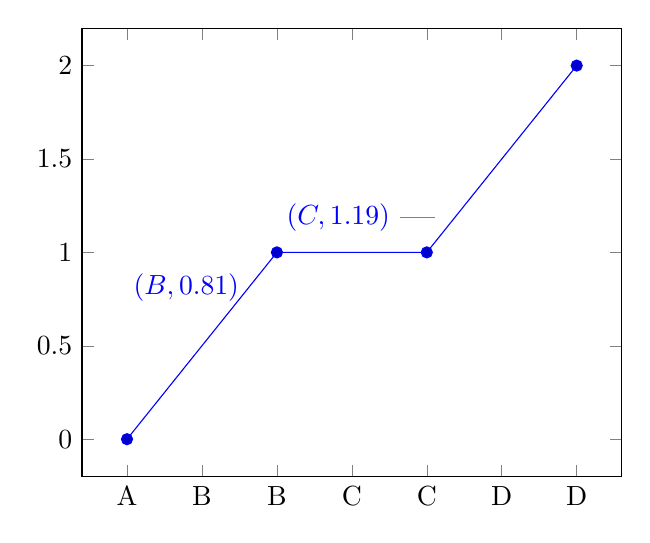
\begin{tikzpicture}
	\begin{axis}[symbolic x coords={A,B,C,D}]
\addplot coordinates {(A,0) (B,1) (C,1) (D,2)} 
	[left]
node[pos=0.3] {%
  \pgfplotspointplotattime
  $(\pgfkeysvalueof{/data point/x},
    \pgfmathprintnumber
		{\pgfkeysvalueof{/data point/y}})$
}
node[pos=0.7,pin=180:{%
  \pgfplotspointplotattime{0.7}
  $(\pgfkeysvalueof{/data point/x},
    \pgfmathprintnumber
		{\pgfkeysvalueof{/data point/y}})$
}] {}
	;
	\end{axis}
\end{tikzpicture}
\end{document}
